\documentclass[12pt, twoside]{article}
% \documentclass[12pt, twoside]{article}
\usepackage[letterpaper, margin=1in, headsep=0.2in]{geometry}
\setlength{\headheight}{0.6in}
%\usepackage[english]{babel}
\usepackage[utf8]{inputenc}
\usepackage{microtype}
\usepackage{amsmath}
\usepackage{amssymb}
%\usepackage{amsfonts}
\usepackage[nomessages]{fp} %\FPeval{\var-name}{2*sin(pi/6)}
\usepackage{siunitx} %units in math. eg 20\milli\meter
\usepackage{yhmath} % for arcs, overparenth command
\usepackage{tikz} %graphics
\usetikzlibrary{quotes, angles, arrows, arrows.meta}
\usepackage{graphicx} %consider setting \graphicspath{{images/}}
\usepackage{parskip} %no paragraph indent
\usepackage{enumitem}
\usepackage{multicol}
\usepackage{venndiagram}

\usepackage{fancyhdr}
\pagestyle{fancy}
\fancyhf{}
\renewcommand{\headrulewidth}{0pt} % disable the underline of the header
\raggedbottom
\hfuzz=2mm %suppresses overfull box warnings

\usepackage{hyperref}
\usepackage{float}

\title{IB Math AA SL}
\author{Chris Huson}
\date{January 2026}

\fancyhead[LE]{\thepage}
\fancyhead[RO]{\thepage \\ First \& last name: \hspace{2.25cm} \,\\ Grade: \hspace{2.25cm} \,}
%\fancyhead[RO]{First \& last name: \hspace{2.25cm} \,\\ \,}
\fancyhead[LO]{La Scuola d'Italia / Huson / IB Math: Probability \\* 16 January 2026}

\begin{document}

\subsubsection*{8.6 Pop Quiz: Rational functions}
\begin{enumerate}[itemsep=0.1cm]

\item Consider the function $\displaystyle f(x)= \frac {2x+3}{3x-6}$ with $x \ne 2$.
    \begin{enumerate}[itemsep=1.0cm]
        \item Write down the equation for the horizontal asymptote.
        \item Write down the equation for the vertical asymptote.
        \item Find the $x$-intercept of the function.
        \item Find the $y$-intercept of the function.
        \item Graph the function $f$, labeling the features identified in the prior questions. 
    \end{enumerate}

\begin{figure}[!htbp]
\begin{center}
\begin{tikzpicture}[scale=1.0]

%grid
\draw [thick, color=black,, xstep=1.0cm,ystep=1.0cm] (-5.5,-5.5) grid (5.5,6.5);
\draw [thin, color=lightgray,, xstep=0.2cm,ystep=0.2cm] (-5.5,-5.5) grid (5.5,6.5);

\foreach \x in {-5, -4, -3, -2, -1, 0,1,2,3,4,5}
\draw[shift={(\x,0)},color=black] (0pt,-1pt) -- (0pt,3pt) node[below]  {$\quad \x$};

\foreach \y in {-5,-4, -3, -2,-1,0,1,2,3,4, 5, 6}
\draw[shift={(0,\y)},color=black] (2pt,0pt) -- (-2pt,0pt) node[left]  {$\y$};

\draw [thick, ->] (-5.5,0) -- (+5.7,0) node [right] {$x$};
\draw [thick, ->] (0,-4.5) -- (0,6.7) node [left] {$y$};

%\draw [<-, ->] plot[domain= -3.5:2.5] (\x, \x*\x +\x -2);
%\draw [<-, ->] plot[domain= -5.5:3] (\x, \x+2);

\end{tikzpicture}
\end{center}
\end{figure}

\newpage
\item Let $f(x) = x^2$ and $g(x)=2x-3$
\begin{enumerate}
    \item Find $(f \circ g)(x)$ \vspace{2.5cm}
    \item Find $g^{-1}(x)$ \vspace{3cm}
    \item Graph and label $f(x)$ on the axes below. Graph and label $f^{-1}(x)$ for $x \geq 0$.
\end{enumerate}

\begin{figure}[!htbp]
\begin{center}
\begin{tikzpicture}

grid
\draw [thin, color=lightgray, xstep=1.0cm,ystep=1.0cm] (-2.1,-2.1) grid (10.1,10.1);
%\draw [, xstep=0.2cm,ystep=0.2cm] (-5.5,-1.5) grid (5.5,16.5);

\foreach \x in {-2, -1, 0,1,2,3,4,5,6,7,8,9,10}
\draw[shift={(\x,0)},color=black] (0pt,-3pt) -- (0pt,3pt) node[below]  {$\x$};

\foreach \y in {-2, -1,0,1,...,10}
\draw[shift={(0,\y)},color=black] (2pt,0pt) -- (-2pt,0pt) node[left]  {$\y$};

\draw [thick, ->] (-2.5,0) -- (+10.5,0) node [right] {$x$};
\draw [thick, ->] (0,-2.0) -- (0,10.5) node [left] {$y$};


\end{tikzpicture}
\end{center}
\end{figure}

\end{enumerate}

\end{document}